\documentclass[12pt]{beamer}
\usepackage[utf8]{inputenc}
\usepackage[T1]{fontenc}
\usepackage{overpic}
\usepackage{rotating}
\usepackage{lmodern}
\usetheme{CambridgeUS}
\begin{document}
	\author{Yerbol Palzhanov}
	\title[MATH 6397]{RPCA for Modal Decomposition of Corrupt Fluid Flows}
	\subtitle{Review of paper by \textit{Scherl et. al.}  }
	\logo{
\includegraphics[width=1cm]{uh.pdf}}
	\institute{University Of Houston}
	%\date{}
	%\subject{MATH 6397}
	%\setbeamercovered{transparent}
	\setbeamertemplate{navigation symbols}{}
	\begin{frame}[plain]
		\maketitle
	\end{frame}
	
	\begin{frame}
		\frametitle{Motivation}
		\begin{figure}
		\begin{center}
			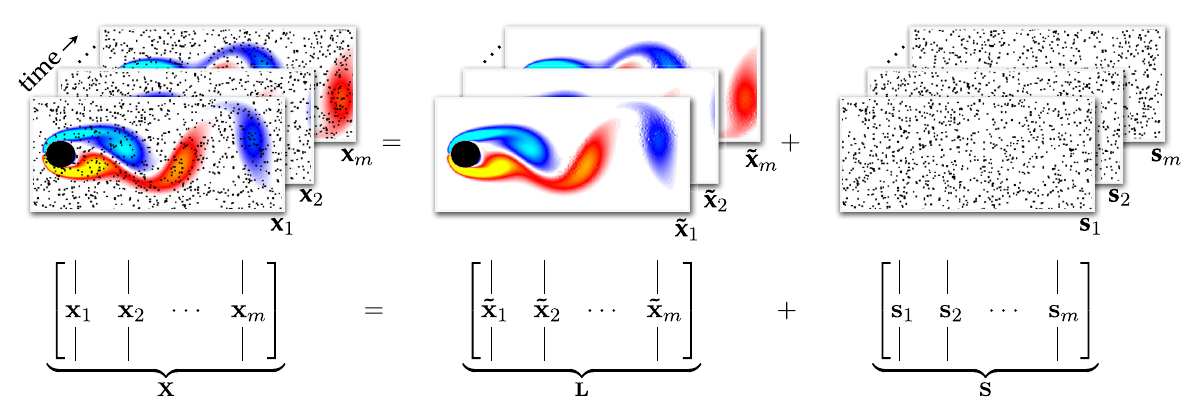
\includegraphics[width=10cm]{./figures/fig01schematic.png}
			\caption{Schematic of RPCA filtering applied to corrupt flow field data.  Corrupted snapshots are arranged as column vectors in the matrix ${\bf X}$, which is decomposed into the sum of a low-rank matrix ${\bf L}$ and a sparse matrix of outliers ${\bf S}$.}
		\end{center}
		\end{figure}
	\end{frame}

	\begin{frame}
	\frametitle{Outline}
	\begin{itemize}
		\item Overview of standard POD and DMD
		\item Robust PCA
		\item Description of flow fields
		\item Results of RPCA filtering
	\end{itemize}
	\end{frame}



	\begin{frame}
		\frametitle{Outline}
		\begin{itemize}
			\item {\color{red}Overview of standard POD and DMD}
			\item Robust PCA
			\item Description of flow fields
			\item Results of RPCA filtering
		\end{itemize}
	\end{frame}


	\begin{frame}
	\frametitle{Proper orthogonal decomposition}
	There are several variants of POD , paper presents a variant of the \textit{snapshot
	POD} of Sirovich that relies on the numerically stable SVD. \\
POD modes are obtained by computing the SVD of ${{\bf X}\in\mathbb{R}^{n\times m}}$:
\begin{align}\label{Eq:SVD}
{\bf X}&={\bf U}\boldsymbol{\Sigma}{\bf V}^T,
\end{align}
where , ${\bf U}\in {\mathbb{R}}^{n\times n}$, $\boldsymbol{\Sigma}\in {\mathbb{R}}^{n\times m}$ and ${\bf V}\in {\mathbb{R}}^{m\times m}$.   
The columns of ${\bf U}$ are \emph{POD modes} with the same dimension as a flow field ${\bf x}$. 
POD modes are orthonormal so that ${\bf U}^T{\bf U} = {\bf I}$; similarly ${\bf V}^T{\bf V} = {\bf I}$.  
Moreover, the columns of ${\bf U}$ (resp. rows of ${\bf V}^T$) are arranged in order of their importance in describing the data. 
\end{frame}


\begin{frame}
	\frametitle{Proper orthogonal decomposition}
The matrix ${\bf X}$ will exhibit \emph{low-rank structure}, so that it is well approximated by the first $r\ll m<n$ columns of ${\bf U}$ and ${\bf V}$:
\begin{align}\label{Eq:SVD2}
{\bf X}&\approx{\bf U}_r\boldsymbol{\Sigma}_r{\bf V}_r^T,
\end{align}
The Eckart-Young theorem states that this is the \emph{optimal} rank-$r$ approximation of the matrix ${\bf X}$ in a least-squares sense. 
\end{frame}


\begin{frame} 
	\frametitle{Dynamic mode decomposition}
	DMD is a modal decomposition technique that simultaneously identifies spatially coherent
	modes that are constrained to have the same linear behavior in time, given by oscillations at a
	fixed frequency with growth or decay\\
	DMD seeks to identify the leading eigenvalues and eigenvectors of the best-fit linear operator ${\bf A}$ that evolves snapshots forward in time:
	%
	\begin{align}
	\textbf{x}_{k+1} \approx \textbf{A} \textbf{x}_k.\label{Eq:DMD:Propagator}
	\end{align}
\end{frame}


\begin{frame} 
	\frametitle{Dynamic mode decomposition}
	\begin{center}
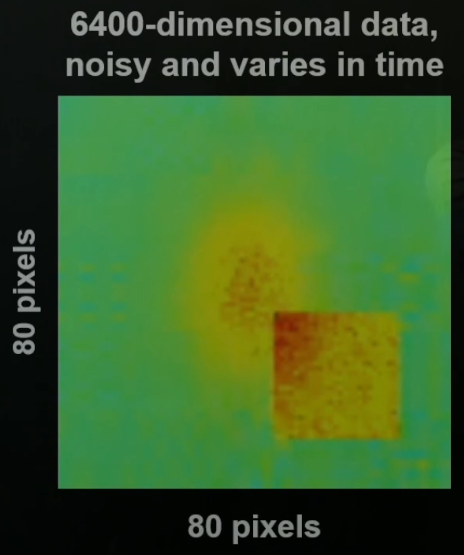
\includegraphics[height=7cm]{./figures/fig1.png}
	\end{center}

\end{frame}


\begin{frame} 
	\frametitle{Dynamic mode decomposition}
	\begin{center}
		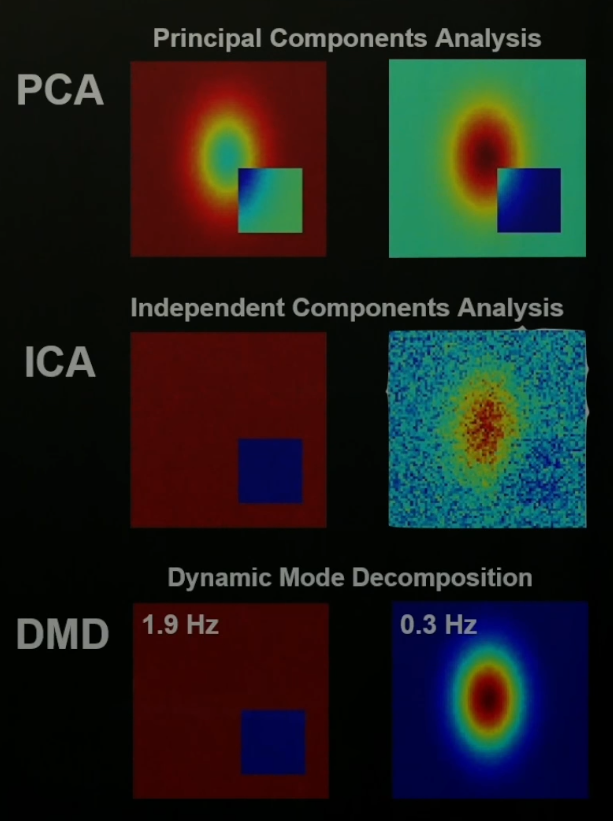
\includegraphics[height=7cm]{./figures/fig2.png}
	\end{center}
	
\end{frame}

	\begin{frame}
	\frametitle{Outline}
	\begin{itemize}
		\item Overview of standard POD and DMD
		\item {\color{red}Robust PCA}
		\item Description of flow fields
		\item Results of RPCA filtering
	\end{itemize}
\end{frame}

\begin{frame} 
	\frametitle{Robust PCA filtering	}
Mathematically, the goal is to find ${\bf L}$ and ${\bf S}$ that satisfy the following:
%
\begin{equation}
\min_{{\bf L},{\bf S}}\text{rank}({\bf L}) + \|{\bf S}\|_0 \,\,\,  \text{subject to} \,\,\, {\bf L} + {\bf S} = {\bf X}.\label{Eq:RPCA:L0}
\end{equation}
%

	
\end{frame}

\begin{frame} 
	\frametitle{Robust PCA filtering	}
	It is possible to solve for ${\bf L}$ and ${\bf S}$ with \emph{high probability} using a convex relaxation of \eqref{Eq:RPCA:L0}:
	%
	\begin{equation}
	\min_{{\bf L},{\bf S}}\|{\bf L}\|_* + \lambda_0\|{\bf S}\|_1 \,\,\,  \text{subject to} \,\,\, {\bf L} + {\bf S} = {\bf X},\label{Eq:RPCA:L1}
	\end{equation}
	%
	where $\|\cdot\|_*$ is the nuclear norm, given by the sum of singular values which is a proxy for the rank of the matrix and ${\lambda_0=\lambda/\sqrt{\max(n,m)}}$ and $\|\cdot\|_1$ is the 1-norm of the matrix. 
	
\end{frame}

\begin{frame} 
	\frametitle{Robust PCA filtering	}

The convex problem in \eqref{Eq:RPCA:L1} is known as \emph{principal component pursuit} (PCP), and may be solved using the augmented Lagrange multiplier (ALM) algorithm.  
	
\end{frame}

\begin{frame} 
	\frametitle{Robust PCA filtering	}
	
Specifically, an augmented Lagrangian may be constructed:
%
\begin{equation}
\mathcal{L}({\bf L},{\bf S},{\bf Y}) = \|{\bf L}\|_* + \lambda_0\|{\bf S}\|_1 + \langle{\bf Y},{\bf X}-{\bf L}-{\bf S}\rangle + \frac{\upsilon}{2}\|{\bf X}-{\bf L}-{\bf S}\|_F^2.
\end{equation}
%
Where $Y$ is the matrix of Lagrange multipliers and $\upsilon$ is a hyperparameter. 
We then solve for ${\bf L}_k$ and ${\bf S}_k$ to minimize $\mathcal{L}$, update the Lagrange multipliers 
\begin{align*}
{\bf Y}_{k+1} = {\bf Y}_k + \upsilon({\bf X}-{\bf L}_k-{\bf S}_k),
\end{align*}
and iterate until convergence.
	
\end{frame}

	\begin{frame}
	\frametitle{Outline}
	\begin{itemize}
		\item Overview of standard POD and DMD
		\item Robust PCA
		\item {\color{red}Description of flow fields}
		\item Results of RPCA filtering
	\end{itemize}
\end{frame}

\begin{frame} \frametitle{Flow fields}
	\begin{figure}
		%\vspace{.075in}
		\begin{center}
			\begin{overpic}[width=.9\textwidth]{figures/fig02modelproblemsc}
				\small
				\put(1,70.2){\textbf{\small Flow past a cylinder, DNS}}
				\put(1,38.5){\textbf{\small Flow past a cylinder, PIV}}
				\put(60,38.5){\textbf{\small Turbine wake, PIV}}
				\put(60.5,70.2){\textbf{\small Channel flow, DNS}}
			\end{overpic}
			\vspace{-.15in}
			\caption{ Example flow field data. }\label{Fig:ModelProblems}
		\end{center}
		\vspace{-.15in}
	\end{figure}
\end{frame}

	\begin{frame}
	\frametitle{Outline}
	\begin{itemize}
		\item Overview of standard POD and DMD
		\item Robust PCA
		\item Description of flow fields
		\item {\color{red}Results of RPCA filtering}
	\end{itemize}
\end{frame}


\end{document}